\question
{\center \bf Medical Image Encryption and Decryption using XOR and PRNGs\\}

A clinic has to send medical images to another institution, but they are
concerned about the safety of the images in transit. They have requested
your help to develop a solution to secure the images so that they cannot
be intercepted or accessed by unauthorized individuals.

\hypertarget{project-requirements}{%
\paragraph{Project Requirements}\label{project-requirements}}

Your task is to create a program that will encrypt the medical images
using XOR and pseudo-random number generator (PRNG) and then save the encrypted images to a safe
location. You will then decrypt the encrypted images using the same
function to ensure that the original images are restored.

To achieve this, you will need to complete the following steps:

\begin{itemize}
\item
  \textbf{Task 1} Read the list of medical images from the given directory. \href{https://ydjemmada.github.io/projects/proj2_images.rar}{Download the set of images from here}
  \begin{figure}[H]
    \centering
    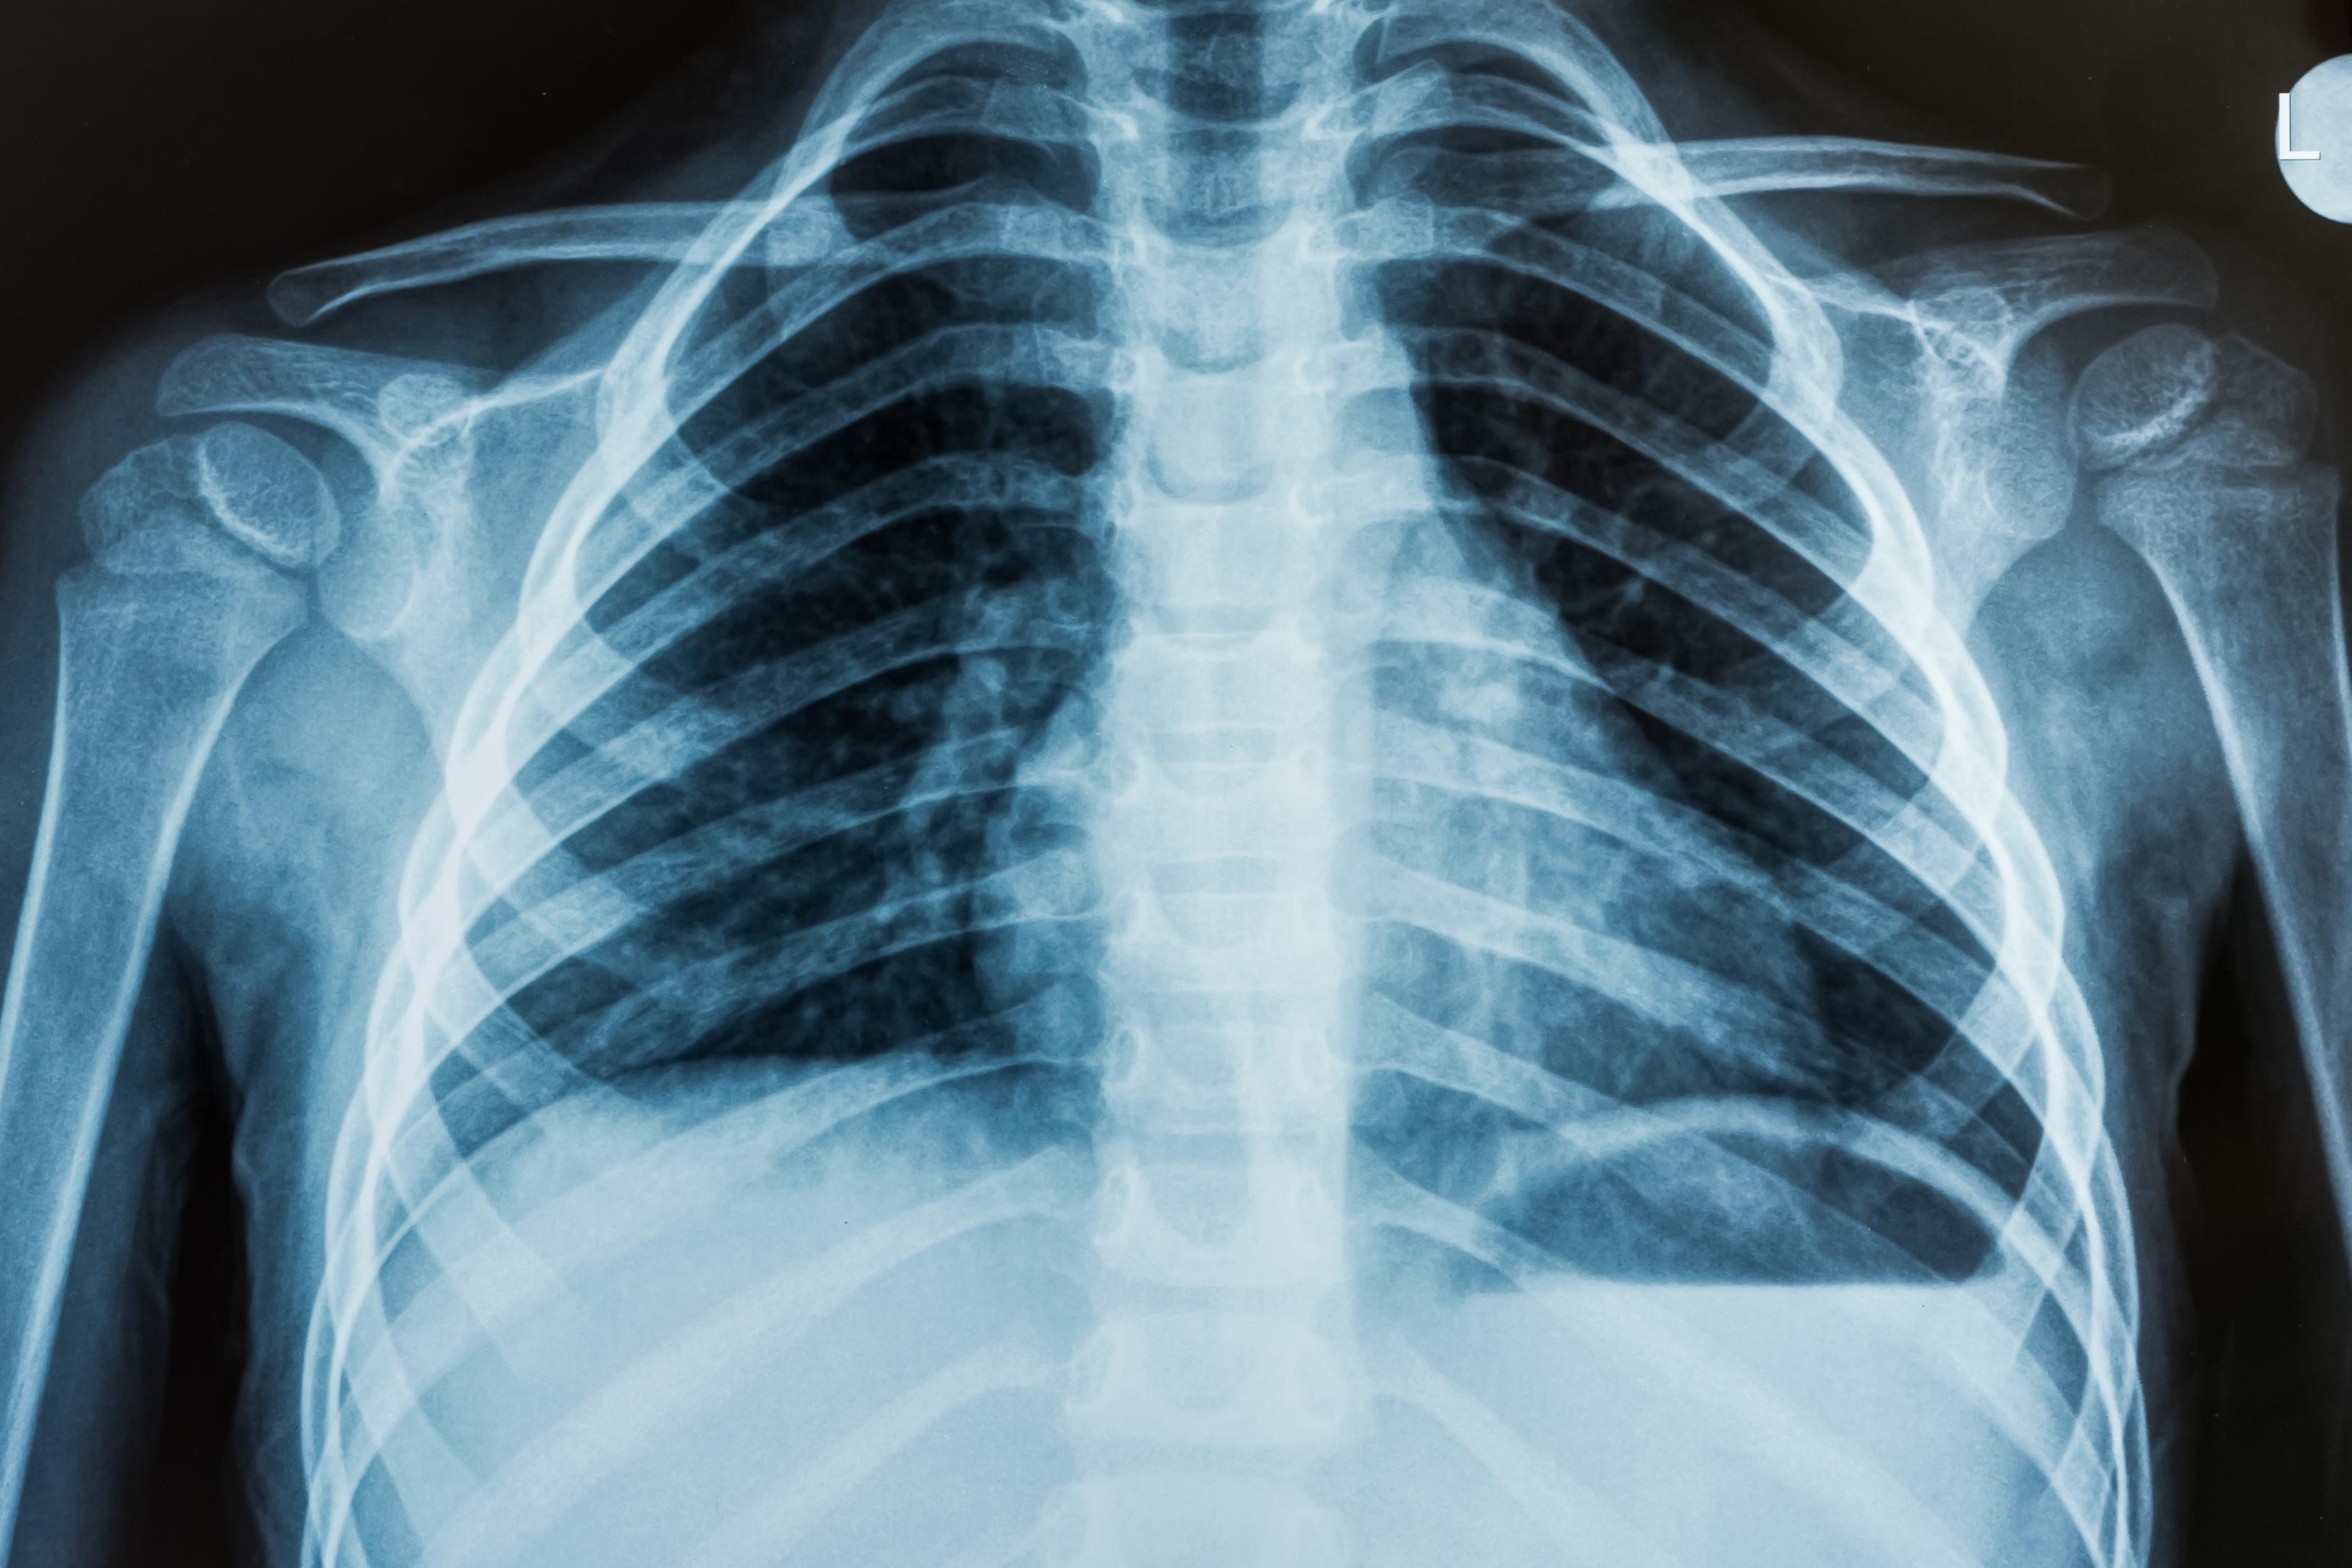
\includegraphics[width=150px]{med_1.jpg} 
  \end{figure}
  \item
  \textbf{Task 2} Implement with python three PRNGs using any of the PRNG algorithms
  available (e.g., Lehmer generator).
  \href{https://en.wikipedia.org/wiki/List_of_random_number_generators}{List
  of prngs}
\item
  \textbf{Task 3} For each medical image, encrypt the image using XOR with a list of random numbers generated with the three PRNGs: xor each byte with a byte from the prng output.
  \begin{figure}[H]\centering
    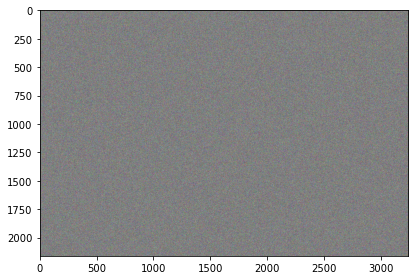
\includegraphics[width=200px]{enc_med_1.png} 
  \end{figure}
\item
  \textbf{Task 4} Save the encrypted image in a folder named \verb|encrypted_data|.
\item
  \textbf{Task 5} For each encrypted image, decrypt the image using the same XOR function and PRNGs (use the same keys as encryption step).
\item
  \textbf{Task 6} Compare the decrypted image with the original image to ensure that the image was decrypted successfully.
\item
  \textbf{Task 7} Write a report on the project, including details on the implementation, the results, and any challenges encountered.
\end{itemize}
\newpage